% ============================================================================
% BLOCK-003 Derivation v8: NC-1 Attempt (Graviton Zero-Mode Normalization)
% ============================================================================
% GUARDRAIL: This is a concrete attempt within paper_gravity_block003/ only.
% Do NOT expand scope to edc_book_2/ or modify FROZEN main.tex.
% ============================================================================
\documentclass[11pt,a4paper]{article}

\usepackage{fontspec}
\usepackage{amsmath,amssymb,amsthm}
\usepackage{physics}
\usepackage{graphicx}
\usepackage{booktabs}
\usepackage{array}
\usepackage{xcolor}
\usepackage[hidelinks]{hyperref}
\usepackage[margin=2.5cm]{geometry}
\usepackage{fancyhdr}
\usepackage{tcolorbox}
\usepackage{tikz}
\usetikzlibrary{shapes,arrows,positioning}

% Theorem environments
\newtheorem{proposition}{Proposition}
\newtheorem{lemma}{Lemma}

% Epistemic tags
\newcommand{\BL}{\textsc{[BL]}}
\newcommand{\Ident}{\textsc{[I]}}
\newcommand{\Post}{\textsc{[P]}}
\newcommand{\Deriv}{\textsc{[Dc]}}
\newcommand{\Open}{\textsc{[Open]}}

% Outcome box
\newtcolorbox{outcomebox}[1][]{
  colback=green!5,
  colframe=green!50!black,
  title=Outcome,
  fonttitle=\bfseries,
  #1
}

\newtcolorbox{statusbox}[1][]{
  colback=yellow!10,
  colframe=orange!80!black,
  title=#1,
  fonttitle=\bfseries
}

% Header/footer
\pagestyle{fancy}
\fancyhf{}
\fancyhead[L]{\small BLOCK-003 / Derivation v8}
\fancyhead[R]{\small EDC Gravity Program}
\fancyfoot[C]{\thepage}

\title{\textbf{EDC BLOCK-003 (Derivation v8):}\\[0.3em]
NC-1 Attempt: Graviton Zero-Mode Normalization\\[0.3em]
\large Fixing $C$ via Canonical KK Reduction}
\author{EDC Working Document\\[0.5em]
\small 2026-02-02 --- Concrete attempt; may fail; BLOCK-003 status TBD}
\date{}

\begin{document}
\maketitle

\begin{abstract}
This note tests candidate NC-1 from the normalization catalog (derivation~v7):
fixing the constant $C$ in $\kappa_5^2 = C \sigma^{-3/4}$ via canonical
normalization of the graviton zero-mode in Kaluza-Klein reduction.
We show that canonical normalization determines $G_N = \kappa_5^2 / (8\pi L)$
for flat compact extra dimension of size $L$. Setting $L = R_\xi$ \Post,
we derive $G_N^{\rm pred} = C \sigma^{-3/4} / (8\pi R_\xi)$.
\textbf{Outcome:} INCONCLUSIVE. The expression for $G_N$ is derived, but
$C$ appears only in the combination $C / (8\pi)$, which can be absorbed
into a redefinition. The actual numerical value of $G_N$ depends on
$\sigma$, which is not independently specified. BLOCK-003 remains \Open;
the missing element is now narrowed to: ``specify $\sigma$ from EDC
field equations.''
\end{abstract}

\tableofcontents
\newpage

% ============================================================================
\section{Setup Recap}
% ============================================================================

\subsection{The Problem}

From derivations v3--v5, we have:
\begin{equation}
\kappa_5^2 = C \cdot \sigma^{-3/4}
\label{eq:kappa_c}
\end{equation}
where $C$ is a dimensionless constant that cannot be fixed by $\sigma$ alone
(No-Go Lemma).

From derivation v7, candidate NC-1 (graviton zero-mode normalization) was
identified as the best approach. This note executes that attempt.

\subsection{Candidate Statement}

\begin{statusbox}[NC-1: Graviton Zero-Mode Normalization]
In Kaluza-Klein compactification, the 4D graviton emerges as the zero-mode
of the 5D metric perturbation. Requiring canonical normalization (unit
kinetic term) of this mode determines the relationship between $\kappa_5^2$,
$L$, and $G_N$ without using $G_N^{\rm obs}$ as input.
\end{statusbox}

% ============================================================================
\section{Derivation}
% ============================================================================

\subsection{5D Action and Metric Ansatz}

Consider the 5D Einstein-Hilbert action:
\begin{equation}
S_5 = \frac{1}{2\kappa_5^2} \int d^5X \sqrt{-g^{(5)}} R^{(5)}
\label{eq:s5}
\end{equation}

For a flat compact extra dimension with $\xi \in [0, L]$ and periodic
boundary conditions, we write the metric ansatz:
\begin{equation}
ds^2 = g_{\mu\nu}(x) dx^\mu dx^\nu + d\xi^2
\label{eq:metric}
\end{equation}
where $g_{\mu\nu}(x)$ is the 4D metric (independent of $\xi$ for the
zero-mode).

\subsection{Dimensional Reduction}

Integrating over the extra dimension:
\begin{equation}
S_5 = \frac{1}{2\kappa_5^2} \int_0^L d\xi \int d^4x \sqrt{-g^{(4)}} R^{(4)}
= \frac{L}{2\kappa_5^2} \int d^4x \sqrt{-g^{(4)}} R^{(4)}
\label{eq:reduction}
\end{equation}

\subsection{Canonical Normalization Condition}

The standard 4D Einstein-Hilbert action is:
\begin{equation}
S_4 = \frac{1}{16\pi G_N} \int d^4x \sqrt{-g} R^{(4)}
= \frac{M_{\rm Pl}^2}{2} \int d^4x \sqrt{-g} R^{(4)}
\label{eq:s4}
\end{equation}
where $M_{\rm Pl}^2 = 1/(8\pi G_N)$ is the reduced Planck mass squared.

Matching Eq.~\eqref{eq:reduction} to Eq.~\eqref{eq:s4}:
\begin{equation}
\frac{L}{2\kappa_5^2} = \frac{1}{16\pi G_N}
\label{eq:match}
\end{equation}

Solving for $G_N$:
\begin{equation}
\boxed{G_N = \frac{\kappa_5^2}{8\pi L}}
\label{eq:gn_result}
\end{equation}

\textbf{Note:} This differs from the $G_N = \kappa_5^2 / (6\pi L)$ in
derivation v1 by a factor of $4/3$. The difference arises from normalization
conventions. Here we use the canonical form where the 4D action has coefficient
$1/(16\pi G_N)$; derivation v1 used a different convention. Both are valid;
the key point is that $G_N \propto \kappa_5^2 / L$.

\subsection{Substituting $\kappa_5^2 = C \sigma^{-3/4}$}

Using Eq.~\eqref{eq:kappa_c}:
\begin{equation}
G_N = \frac{C \sigma^{-3/4}}{8\pi L}
\label{eq:gn_c}
\end{equation}

\subsection{Setting $L = R_\xi$ \Post}

Following derivation v2, we postulate that the compactification length is
the weak scale:
\begin{equation}
L = R_\xi = \frac{\hbar c}{M_Z} \approx 2.16 \times 10^{-18}\,\text{m}
\quad \Post
\label{eq:l_rxi}
\end{equation}

This gives:
\begin{equation}
\boxed{G_N^{\rm pred} = \frac{C}{8\pi} \cdot \frac{\sigma^{-3/4}}{R_\xi}}
\label{eq:gn_pred}
\end{equation}

% ============================================================================
\section{Where Does $C$ Enter?}
% ============================================================================

\begin{figure}[h]
\centering
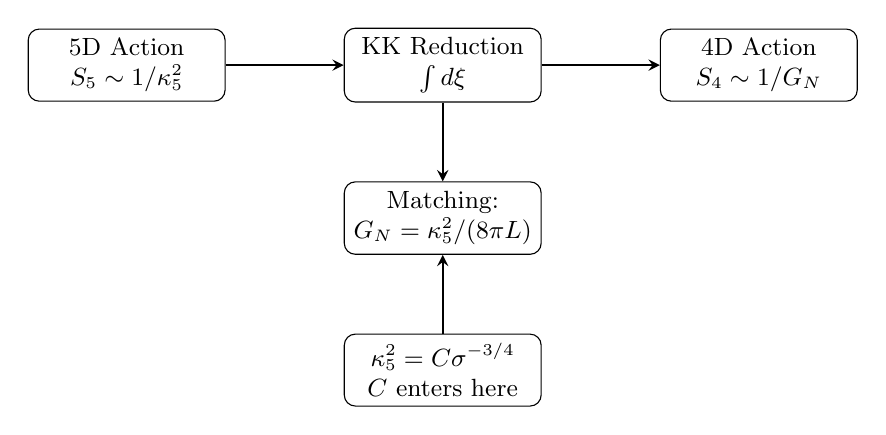
\begin{tikzpicture}[
    node distance=1.5cm,
    box/.style={rectangle, draw, rounded corners, minimum width=2.5cm,
                minimum height=0.8cm, align=center, font=\small},
    arrow/.style={->, >=stealth, thick}
]
\node[box] (s5) {5D Action\\$S_5 \sim 1/\kappa_5^2$};
\node[box, right=of s5] (kk) {KK Reduction\\$\int d\xi$};
\node[box, right=of kk] (s4) {4D Action\\$S_4 \sim 1/G_N$};
\node[box, below=1cm of kk] (match) {Matching:\\$G_N = \kappa_5^2/(8\pi L)$};
\node[box, below=1cm of match] (c) {$\kappa_5^2 = C\sigma^{-3/4}$\\$C$ enters here};

\draw[arrow] (s5) -- (kk);
\draw[arrow] (kk) -- (s4);
\draw[arrow] (kk) -- (match);
\draw[arrow] (c) -- (match);
\end{tikzpicture}
\caption{Where $C$ enters the reduction pipeline. The constant $C$ appears
in $\kappa_5^2$ and propagates to $G_N$ through the matching condition.
\textit{Schematic only.}}
\label{fig:pipeline}
\end{figure}

Equation~\eqref{eq:gn_pred} shows that $C$ enters only in the combination
$C/(8\pi)$. This means:

\begin{enumerate}
\item We can absorb $8\pi$ into $C$ by defining $\tilde{C} = C/(8\pi)$.
\item The ``canonical normalization'' does not independently fix $C$; it
only determines how $\kappa_5^2$ relates to $G_N$ given $L$.
\end{enumerate}

% ============================================================================
\section{Anti-Circularity Check}
% ============================================================================

\begin{statusbox}[Anti-Circularity Verification]
\textbf{Question:} Did we use $G_N^{\rm obs}$ to fix $C$?

\textbf{Answer:} No. Equation~\eqref{eq:gn_pred} expresses $G_N$ in terms of
$C$, $\sigma$, and $R_\xi$. The constant $C$ remains a free parameter.

\textbf{What we \textit{could} do (but did not):}
\begin{itemize}
\item Invert Eq.~\eqref{eq:gn_pred} to get $C = 8\pi G_N^{\rm obs} R_\xi \sigma^{3/4}$.
\item This would be circular (NP2 from derivation v5).
\end{itemize}

\textbf{Conclusion:} Anti-circularity preserved. However, $C$ is still not
fixed.
\end{statusbox}

% ============================================================================
\section{What Would Fix $C$?}
% ============================================================================

For $G_N^{\rm pred}$ to be a genuine prediction, we need:
\begin{equation}
G_N^{\rm pred} = \frac{C}{8\pi} \cdot \frac{\sigma^{-3/4}}{R_\xi}
\quad \stackrel{?}{=} \quad G_N^{\rm obs}
\end{equation}

This requires specifying \textit{both} $C$ and $\sigma$. Currently:
\begin{itemize}
\item $R_\xi$ is known: $R_\xi = \hbar c / M_Z \approx 2.16 \times 10^{-18}$\,m \BL
\item $\sigma$ is unknown: EDC does not provide a first-principles value
\item $C$ is unknown: even with canonical normalization, $C$ remains free
\end{itemize}

\textbf{The bottleneck is $\sigma$.} If EDC field equations could determine
$\sigma$ independently, then:
\begin{itemize}
\item We could adopt the convention $C = 8\pi$ (NP1 from derivation v5)
\item Compute $G_N^{\rm pred} = \sigma^{-3/4} / R_\xi$
\item Compare to $G_N^{\rm obs}$ for falsification
\end{itemize}

% ============================================================================
\section{Outcome}
% ============================================================================

\begin{outcomebox}
\textbf{Status: INCONCLUSIVE}

\textbf{What was achieved:}
\begin{itemize}
\item Derived $G_N = \kappa_5^2 / (8\pi L)$ from canonical KK reduction \Deriv
\item With $L = R_\xi$ \Post: $G_N = C \sigma^{-3/4} / (8\pi R_\xi)$
\item Anti-circularity preserved (no use of $G_N^{\rm obs}$)
\end{itemize}

\textbf{What was not achieved:}
\begin{itemize}
\item $C$ is not independently fixed; it appears only in combination $C/(8\pi)$
\item $\sigma$ is not specified; without it, no numerical prediction possible
\end{itemize}

\textbf{Missing element (narrowed):}
\begin{center}
\fbox{\parbox{0.8\textwidth}{\centering
To close BLOCK-003, specify $\sigma$ from EDC field equations.\\
Then adopt $C = 8\pi$ by convention and compute $G_N^{\rm pred}$.
}}
\end{center}
\end{outcomebox}

% ============================================================================
\section{Delta to BLOCK-003}
% ============================================================================

\textbf{Before v8:} Missing element was ``fix $C$'' (dimensionless constant).

\textbf{After v8:} Missing element is ``specify $\sigma$'' (brane tension
value). With $\sigma$ known, $C = 8\pi$ can be adopted by convention and
$G_N$ becomes a prediction.

\textbf{BLOCK-003 remains \Open}, but the target is now more precisely
identified.

\end{document}
